\documentclass[border=4pt,12pt]{standalone}
% House style for redrawn exam diagrams (diagram-v4: 0.4pt lines, filled -latex arrows, fine dashes; stipple and hatching drawn as real dots/lines (no PDF/SVG patterns, so they render in every browser and at any scale); transparent background). Every figure \input's this.
\usepackage{amsmath,amssymb}
\usepackage{txfonts}
\usepackage{pdfrender,xcolor}
% \halo{text}: label on shading. The shading stops just around each letter's outline (a thin knock-out that follows the
% glyphs, like the papers' typesetting), never a box. Owner: "I don't want a box around the text".
\newcommand{\halo}[1]{\leavevmode\rlap{\pdfrender{TextRenderingMode=2,LineWidth=2.2pt,LineJoinStyle=1,StrokeColor=white,FillColor=white}#1}#1}
\usepackage{tikz,pgfplots}
\pgfplotsset{compat=1.18}
\usetikzlibrary{arrows.meta,calc,angles,quotes,patterns,patterns.meta,intersections,positioning,decorations.markings,shapes.geometric}
% Stipple and hatching are drawn as actual dots / lines clipped to the region (path picture), NOT as pattern fills:
% SVG <pattern> fills vanish or blur when browsers scale the image, so the owner could not see the shading.
% Each dot is a 0.72pt square (keeps SVGs small; reads as a dot at print size). Dots sit on one global staggered grid, so neighbouring regions line up.
\makeatletter
\newdimen\ex@x \newdimen\ex@y \newdimen\ex@xa \newdimen\ex@ya \newdimen\ex@xb \newdimen\ex@yb \newcount\ex@row
\def\exam@stipplecolor{black!75}\def\exam@dotr{0.42pt}\def\exam@dotgap{2.5}
\def\ex@rowdots{\ifdim\ex@x<\ex@xb \pgfpathrectangle{\pgfqpoint{\dimexpr\ex@x-0.36pt\relax}{\dimexpr\ex@y-0.36pt\relax}}{\pgfqpoint{0.72pt}{0.72pt}}\advance\ex@x by \exam@dotgap pt\relax\expandafter\ex@rowdots\fi}
\def\exam@stipple{%
  \pgftransformreset% dots are sized in real points even inside scaled pictures
  \pgfpointanchor{path picture bounding box}{south west}\ex@xa=\pgf@x \ex@ya=\pgf@y
  \pgfpointanchor{path picture bounding box}{north east}\ex@xb=\pgf@x \ex@yb=\pgf@y
  \pgfsetfillcolor{\exam@stipplecolor}\pgfmathsetmacro\ex@h{\exam@dotgap/2}%
  \pgfmathtruncatemacro\ex@r{floor(\ex@ya/\ex@h)-1}\ex@row=\ex@r\relax
  \ex@y=\ex@r\dimexpr\ex@h pt\relax
  \loop\ifdim\ex@y<\ex@yb
    \pgfmathtruncatemacro\ex@c{floor(\ex@xa/\exam@dotgap)-1}\ex@x=\ex@c\dimexpr\exam@dotgap pt\relax
    \ifodd\ex@row \advance\ex@x by \ex@h pt\fi
    \ex@rowdots
    \advance\ex@y by \ex@h pt \advance\ex@row by 1
    \ifnum\numexpr\ex@row-(\ex@row/4)*4\relax=0 \pgfusepath{fill}\fi% flush every 4 rows: bounded TeX memory, few clip copies in the SVG
  \repeat\pgfusepath{fill}}
\newdimen\ex@d
\def\exam@hatch#1{% #1 = 1 for /, -1 for \ ; lines 45 degrees, 3pt apart
  \pgftransformreset
  \pgfpointanchor{path picture bounding box}{south west}\ex@xa=\pgf@x \ex@ya=\pgf@y
  \pgfpointanchor{path picture bounding box}{north east}\ex@xb=\pgf@x \ex@yb=\pgf@y
  \ex@d=\dimexpr\ex@yb-\ex@ya\relax \ex@x=\dimexpr\ex@xa-\ex@d\relax
  \loop\ifdim\ex@x<\ex@xb
    \ifnum#1>0 \pgfpathmoveto{\pgfqpoint{\ex@x}{\ex@ya}}\pgfpathlineto{\pgfqpoint{\dimexpr\ex@x+\ex@d\relax}{\ex@yb}}%
    \else \pgfpathmoveto{\pgfqpoint{\ex@x}{\ex@yb}}\pgfpathlineto{\pgfqpoint{\dimexpr\ex@x+\ex@d\relax}{\ex@ya}}\fi
    \advance\ex@x by 4.24pt
  \repeat
  \pgfsetlinewidth{0.4pt}\pgfsetstrokecolor{black}\pgfusepath{stroke}}
\def\examstipple{\exam@stipple}\def\examhatch{\exam@hatch}\def\examsetstipplecolor#1{\def\exam@stipplecolor{#1}}\def\examsetdotgap#1{\def\exam@dotgap{#1}}
\makeatother
% (legacy pattern kept for old files)
% staggered stipple like the NESA papers' dotted shading
\pgfdeclarepatternformonly{exam stipple}{\pgfpointorigin}{\pgfqpoint{2.2pt}{2.2pt}}{\pgfqpoint{2.2pt}{2.2pt}}{%
  \pgfpathcircle{\pgfqpoint{0.55pt}{0.55pt}}{0.42pt}\pgfpathcircle{\pgfqpoint{1.65pt}{1.65pt}}{0.42pt}\pgfusepath{fill}}
\tikzset{
  every picture/.style={line width=0.6pt, >={Latex[length=2mm,width=1.3mm]}},
  curve/.style={line width=0.6pt},
  open arrow/.style={-{Latex[length=2mm,width=1.3mm]}},  % owner: filled -latex heads everywhere, no open chevrons
  aux/.style={dash pattern=on 2pt off 1.5pt, line width=0.6pt},
  shade/.code={\def\exA{#1}\def\exB{none}\ifx\exA\exB\else\pgfkeysalso{fill=black!18}\fi},
  shade/.default=on,
  shade dots/.style={fill=none, path picture={\examstipple}},
  stipple color/.code={\examsetstipplecolor{#1}},
  stipple gap/.code={\examsetdotgap{#1}},
  shade dense dots/.style={fill=none, stipple gap=1.6, path picture={\examstipple}},
  shade hatch/.style={fill=none, path picture={\examhatch{1}}},
  shade hatch reverse/.style={fill=none, path picture={\examhatch{-1}}},
  shade solid/.style={fill=black},
  pt/.style={circle, fill, inner sep=1.1pt},
  open pt/.style={circle, draw, fill=white, inner sep=1.1pt},
}
\pgfplotsset{
  exam axes/.style={axis lines=middle, axis line style={->}, xlabel={$x$}, ylabel={$y$},
    xlabel style={anchor=west}, ylabel style={anchor=south}, tick label style={font=\small},
    every axis plot/.append style={line width=0.6pt, black}, samples=200, clip=false,
    enlargelimits=false, axis on top},
}

\begin{document}
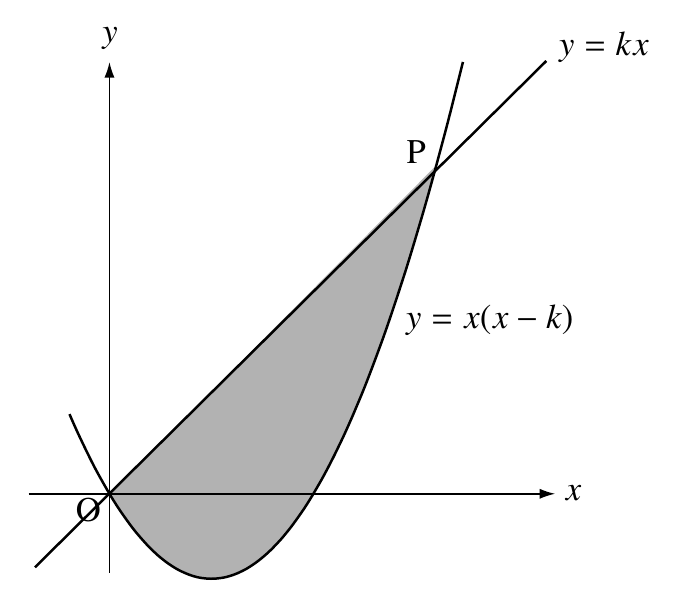
\begin{tikzpicture}[x=0.0127cm,y=-0.0127cm,font=\fontsize{12.5}{15.0}\selectfont]
\fill[black!30] (103,487) -- (430,158.4) -- plot[smooth] coordinates {(430.0,158.4) (424.5,178.5) (418.9,198.1) (413.4,217.3) (407.8,235.9) (402.3,254.0) (396.7,271.6) (391.2,288.7) (385.7,305.3) (380.1,321.5) (374.6,337.1) (369.0,352.2) (363.5,366.8) (357.9,380.9) (352.4,394.5) (346.9,407.6) (341.3,420.2) (335.8,432.3) (330.2,443.9) (324.7,455.0) (319.2,465.5) (313.6,475.6) (308.1,485.2) (302.5,494.3) (297.0,502.9) (291.4,511.0) (285.9,518.5) (280.4,525.6) (274.8,532.2) (269.3,538.3) (263.7,543.8) (258.2,548.9) (252.6,553.5) (247.1,557.5) (241.6,561.1) (236.0,564.1) (230.5,566.7) (224.9,568.8) (219.4,570.3) (213.8,571.4) (208.3,571.9) (202.8,572.0) (197.2,571.5) (191.7,570.6) (186.1,569.1) (180.6,567.1) (175.1,564.7) (169.5,561.7) (164.0,558.2) (158.4,554.3) (152.9,549.8) (147.3,544.8) (141.8,539.4) (136.3,533.4) (130.7,526.9) (125.2,519.9) (119.6,512.5) (114.1,504.5) (108.5,496.0) (103.0,487.0)} -- cycle;
\draw[->] (22,487)--(549,487); \draw[->] (103,566)--(103,55);
\draw[line width=0.9pt] (28.5,560.5)--(540,54);
\draw[line width=0.9pt] plot[smooth] coordinates {(63.0,407.3) (67.4,417.4) (71.8,427.1) (76.3,436.6) (80.7,445.7) (85.1,454.6) (89.5,463.1) (94.0,471.3) (98.4,479.1) (102.8,486.7) (107.2,493.9) (111.6,500.8) (116.1,507.4) (120.5,513.6) (124.9,519.6) (129.3,525.2) (133.8,530.5) (138.2,535.5) (142.6,540.2) (147.0,544.5) (151.4,548.6) (155.9,552.3) (160.3,555.7) (164.7,558.7) (169.1,561.5) (173.5,563.9) (178.0,566.0) (182.4,567.8) (186.8,569.3) (191.2,570.5) (195.7,571.3) (200.1,571.8) (204.5,572.0) (208.9,571.9) (213.3,571.4) (217.8,570.7) (222.2,569.6) (226.6,568.2) (231.0,566.5) (235.5,564.4) (239.9,562.1) (244.3,559.4) (248.7,556.4) (253.1,553.1) (257.6,549.4) (262.0,545.5) (266.4,541.2) (270.8,536.6) (275.3,531.7) (279.7,526.4) (284.1,520.9) (288.5,515.0) (292.9,508.8) (297.4,502.3) (301.8,495.5) (306.2,488.3) (310.6,480.8) (315.1,473.0) (319.5,464.9) (323.9,456.5) (328.3,447.8) (332.7,438.7) (337.2,429.3) (341.6,419.6) (346.0,409.6) (350.4,399.2) (354.9,388.5) (359.3,377.6) (363.7,366.2) (368.1,354.6) (372.5,342.7) (377.0,330.4) (381.4,317.8) (385.8,304.9) (390.2,291.7) (394.6,278.2) (399.1,264.3) (403.5,250.1) (407.9,235.6) (412.3,220.8) (416.8,205.6) (421.2,190.2) (425.6,174.4) (430.0,158.3) (434.4,141.9) (438.9,125.1) (443.3,108.1) (447.7,90.7) (452.1,73.0) (456.6,55.0)};
\node[anchor=base,inner sep=0] at (103.5,36) {$y$}; \node[anchor=base,inner sep=0] at (566.5,494) {$x$};
\node[anchor=base,inner sep=0] at (82,515) {O}; \node[anchor=base,inner sep=0] at (410,157) {P};
\node[anchor=base west,inner sep=0] at (399,322) {$y=x(x-k)$}; \node[anchor=base west,inner sep=0] at (552,49) {$y=kx$};\end{tikzpicture}
\end{document}
